\documentclass{standalone}
\usepackage{tikz}
\usetikzlibrary{arrows.meta}
\begin{document}
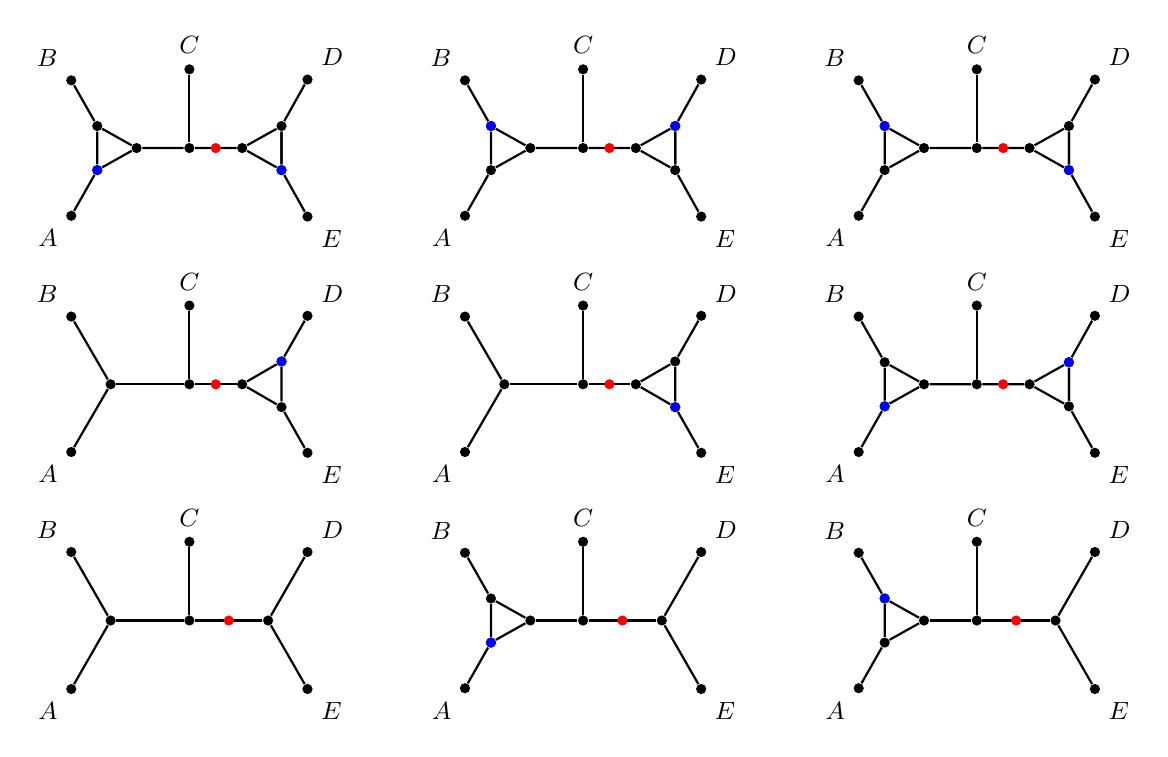
\begin{tikzpicture}[>=Stealth, every node/.style={font=\small},dot/.style={circle,fill=black,inner sep=1.3pt},leaf/.style={dot},int/.style={dot},]
\begin{scope}[shift={(0,0)}]
\node[int] (u) at (0,0) {};
\node[int] (v) at (1,0) {};
\node[int] (w) at (2,0) {};
\node[leaf,label=below left:$A$] (A) at (-0.5,-0.87) {};
\node[leaf,label=above left:$B$] (B) at (-0.5, 0.87) {};
\node[leaf,label=above:$C$] (C) at (1,1) {};
\node[leaf,label=above right:$D$] (D) at (2.5, 0.87) {};
\node[leaf,label=below right:$E$] (E) at (2.5,-0.87) {};
\draw[line width=0.8pt] (A) -- (u) -- (B);
\draw[line width=0.8pt] (u) -- (v) -- (w);
\draw[line width=0.8pt] (v) -- (C);
\draw[line width=0.8pt] (D) -- (w) -- (E);
\node[circle,fill=red,inner sep=1.3pt] (root) at (1.5,0) {};
\end{scope}
\begin{scope}[shift={(5,0)}]
\node[int] (u3) at (0.33,0) {};
\node[int] (u1) at (-0.17,-0.28) {};
\node[int] (u2) at (-0.17,0.28) {};
\node[int] (v) at (1,0) {};
\node[int] (w) at (2,0) {};
\node[leaf, label=below left:$A$] (A) at (-.5, -0.86) {};
\node[leaf, label=above left:$B$] (B) at (-.5, 0.86) {};
\node[leaf, label=above:$C$] (C) at (1,1) {};
\node[leaf, label=above right:$D$] (D) at (2.5,0.87) {};
\node[leaf, label=below right:$E$] (E) at (2.5,-0.87) {};
\draw[line width=0.8pt] (u1) -- (u2) -- (u3) -- (u1);
\draw[line width=0.8pt] (A) -- (u1);
\draw[line width=0.8pt] (B) -- (u2);
\draw[line width=0.8pt] (u3) -- (v) -- (w);
\draw[line width=0.8pt] (C) -- (v);
\draw[line width=0.8pt] (D) -- (w) -- (E);
\node[circle,fill=red,inner sep=1.3pt] (root) at (3/2,0) {};
\node[circle,fill=blue,inner sep=1.3pt] at (-.17,-.28) {};
\end{scope}
\begin{scope}[shift={(10,0)}]
\node[int] (u3) at (0.33,0) {};
\node[int] (u1) at (-0.17,-0.28) {};
\node[int] (u2) at (-0.17,0.28) {};
\node[int] (v) at (1,0) {};
\node[int] (w) at (2,0) {};
\node[leaf, label=below left:$A$] (A) at (-.5, -0.86) {};
\node[leaf, label=above left:$B$] (B) at (-.5, 0.86) {};
\node[leaf, label=above:$C$] (C) at (1,1) {};
\node[leaf, label=above right:$D$] (D) at (2.5,0.87) {};
\node[leaf, label=below right:$E$] (E) at (2.5,-0.87) {};
\draw[line width=0.8pt] (u1) -- (u2) -- (u3) -- (u1);
\draw[line width=0.8pt] (A) -- (u1);
\draw[line width=0.8pt] (B) -- (u2);
\draw[line width=0.8pt] (u3) -- (v) -- (w);
\draw[line width=0.8pt] (C) -- (v);
\draw[line width=0.8pt] (D) -- (w) -- (E);
\node[circle,fill=red,inner sep=1.3pt] (root) at (3/2,0) {};
\node[circle,fill=blue,inner sep=1.3pt] at (-.17,.28) {};
\end{scope}
\begin{scope}[shift={(0,3)}]
\node[int] (u) at (0,0) {};
\node[int] (v) at (1,0) {};
\node[int] (w1) at (1.67,0) {};
\node[int] (w2) at (2.17,0.29) {};
\node[int] (w3) at (2.17,-0.29) {};
\node[leaf, label=below left:$A$] (A) at (-.5, -0.86) {};
\node[leaf, label=above left:$B$] (B) at (-.5, 0.86) {};
\node[leaf, label=above:$C$] (C) at (1,1) {};
\node[leaf, label=above right:$D$] (D) at (2.5,0.87) {};
\node[leaf, label=below right:$E$] (E) at (2.5,-0.87) {};
\draw[line width=0.8pt] (A) -- (u) -- (B);
\draw[line width=0.8pt] (u) -- (v) -- (w1);
\draw[line width=0.8pt] (C) -- (v);
\draw[line width=0.8pt] (w1) -- (w2) -- (w3) -- (w1);
\draw[line width=0.8pt] (w2) -- (D);
\draw[line width=0.8pt] (w3) -- (E);
\node[circle,fill=red,inner sep=1.3pt] at (1.335,0) {};
\node[circle,fill=blue,inner sep=1.3pt] at (2.17,.29) {};
\end{scope}
\begin{scope}[shift={(5,3)}]
\node[int] (u) at (0,0) {};
\node[int] (v) at (1,0) {};
\node[int] (w1) at (1.67,0) {};
\node[int] (w2) at (2.17,0.29) {};
\node[int] (w3) at (2.17,-0.29) {};
\node[leaf, label=below left:$A$] (A) at (-.5, -0.86) {};
\node[leaf, label=above left:$B$] (B) at (-.5, 0.86) {};
\node[leaf, label=above:$C$] (C) at (1,1) {};
\node[leaf, label=above right:$D$] (D) at (2.5,0.87) {};
\node[leaf, label=below right:$E$] (E) at (2.5,-0.87) {};
\draw[line width=0.8pt] (A) -- (u) -- (B);
\draw[line width=0.8pt] (u) -- (v) -- (w1);
\draw[line width=0.8pt] (C) -- (v);
\draw[line width=0.8pt] (w1) -- (w2) -- (w3) -- (w1);
\draw[line width=0.8pt] (w2) -- (D);
\draw[line width=0.8pt] (w3) -- (E);
\node[circle,fill=red,inner sep=1.3pt] at (1.335,0) {};
\node[circle,fill=blue,inner sep=1.3pt] at (2.17,-.29) {};
\end{scope}
\begin{scope}[shift={(10,3)}]
\node[int] (u3) at (0.33,0) {};
\node[int] (u1) at (-0.17,-0.28) {};
\node[int] (u2) at (-0.17,0.28) {};
\node[int] (v) at (1,0) {};
\node[int] (w1) at (1.67,0) {};
\node[int] (w2) at (2.17,0.28) {};
\node[int] (w3) at (2.17,-0.28) {};
\node[leaf, label=below left:$A$] (A) at (-.5, -0.86) {};
\node[leaf, label=above left:$B$] (B) at (-.5, 0.86) {};
\node[leaf, label=above:$C$] (C) at (1,1) {};
\node[leaf, label=above right:$D$] (D) at (2.5,0.87) {};
\node[leaf, label=below right:$E$] (E) at (2.5,-0.87) {};
\draw[line width=0.8pt] (u1) -- (u2) -- (u3) -- (u1);
\draw[line width=0.8pt] (A) -- (u1);
\draw[line width=0.8pt] (B) -- (u2);
\draw[line width=0.8pt] (u3) -- (v) -- (w1) -- (w2) -- (w3) -- (w1);
\draw[line width=0.8pt] (C) -- (v);
\draw[line width=0.8pt] (D) -- (w2) -- (w3) -- (E);
\node[circle,fill=red,inner sep=1.3pt] (root) at (1.335,0) {};
\node[circle,fill=blue,inner sep=1.3pt] at (2.17,.28) {};
\node[circle,fill=blue,inner sep=1.3pt] at (-.17,-.28) {};
\end{scope}
\begin{scope}[shift={(0,6)}]
\node[int] (u3) at (0.33,0) {};
\node[int] (u1) at (-0.17,-0.28) {};
\node[int] (u2) at (-0.17,0.28) {};
\node[int] (v) at (1,0) {};
\node[int] (w1) at (1.67,0) {};
\node[int] (w2) at (2.17,0.28) {};
\node[int] (w3) at (2.17,-0.28) {};
\node[leaf, label=below left:$A$] (A) at (-.5, -0.86) {};
\node[leaf, label=above left:$B$] (B) at (-.5, 0.86) {};
\node[leaf, label=above:$C$] (C) at (1,1) {};
\node[leaf, label=above right:$D$] (D) at (2.5,0.87) {};
\node[leaf, label=below right:$E$] (E) at (2.5,-0.87) {};
\draw[line width=0.8pt] (u1) -- (u2) -- (u3) -- (u1);
\draw[line width=0.8pt] (A) -- (u1);
\draw[line width=0.8pt] (B) -- (u2);
\draw[line width=0.8pt] (u3) -- (v) -- (w1) -- (w2) -- (w3) -- (w1);
\draw[line width=0.8pt] (C) -- (v);
\draw[line width=0.8pt] (D) -- (w2) -- (w3) -- (E);
\node[circle,fill=red,inner sep=1.3pt] (root) at (1.335,0) {};
\node[circle,fill=blue,inner sep=1.3pt] at (2.17,-.28) {};
\node[circle,fill=blue,inner sep=1.3pt] at (-.17,-.28) {};
\end{scope}
\begin{scope}[shift={(5,6)}]
\node[int] (u3) at (0.33,0) {};
\node[int] (u1) at (-0.17,-0.28) {};
\node[int] (u2) at (-0.17,0.28) {};
\node[int] (v) at (1,0) {};
\node[int] (w1) at (1.67,0) {};
\node[int] (w2) at (2.17,0.28) {};
\node[int] (w3) at (2.17,-0.28) {};
\node[leaf, label=below left:$A$] (A) at (-.5, -0.86) {};
\node[leaf, label=above left:$B$] (B) at (-.5, 0.86) {};
\node[leaf, label=above:$C$] (C) at (1,1) {};
\node[leaf, label=above right:$D$] (D) at (2.5,0.87) {};
\node[leaf, label=below right:$E$] (E) at (2.5,-0.87) {};
\draw[line width=0.8pt] (u1) -- (u2) -- (u3) -- (u1);
\draw[line width=0.8pt] (A) -- (u1);
\draw[line width=0.8pt] (B) -- (u2);
\draw[line width=0.8pt] (u3) -- (v) -- (w1) -- (w2) -- (w3) -- (w1);
\draw[line width=0.8pt] (C) -- (v);
\draw[line width=0.8pt] (D) -- (w2) -- (w3) -- (E);
\node[circle,fill=red,inner sep=1.3pt] (root) at (1.335,0) {};
\node[circle,fill=blue,inner sep=1.3pt] at (2.17,.28) {};
\node[circle,fill=blue,inner sep=1.3pt] at (-.17,.28) {};
\end{scope}
\begin{scope}[shift={(10,6)}]
\node[int] (u3) at (0.33,0) {};
\node[int] (u1) at (-0.17,-0.28) {};
\node[int] (u2) at (-0.17,0.28) {};
\node[int] (v) at (1,0) {};
\node[int] (w1) at (1.67,0) {};
\node[int] (w2) at (2.17,0.28) {};
\node[int] (w3) at (2.17,-0.28) {};
\node[leaf, label=below left:$A$] (A) at (-.5, -0.86) {};
\node[leaf, label=above left:$B$] (B) at (-.5, 0.86) {};
\node[leaf, label=above:$C$] (C) at (1,1) {};
\node[leaf, label=above right:$D$] (D) at (2.5,0.87) {};
\node[leaf, label=below right:$E$] (E) at (2.5,-0.87) {};
\draw[line width=0.8pt] (u1) -- (u2) -- (u3) -- (u1);
\draw[line width=0.8pt] (A) -- (u1);
\draw[line width=0.8pt] (B) -- (u2);
\draw[line width=0.8pt] (u3) -- (v) -- (w1) -- (w2) -- (w3) -- (w1);
\draw[line width=0.8pt] (C) -- (v);
\draw[line width=0.8pt] (D) -- (w2) -- (w3) -- (E);
\node[circle,fill=red,inner sep=1.3pt] (root) at (1.335,0) {};
\node[circle,fill=blue,inner sep=1.3pt] at (2.17,-.28) {};
\node[circle,fill=blue,inner sep=1.3pt] at (-.17,.28) {};
\end{scope}
\end{tikzpicture}
\end{document}